\section{Demonstration Outline}
\label{sec:demo}

The objective of this demonstration is to show how \sys can quickly and accurately detect 
and propose fixes to errors in a query log, and compare its results to alternatives
that use existing techniques.


\begin{figure}[t]
\centering
  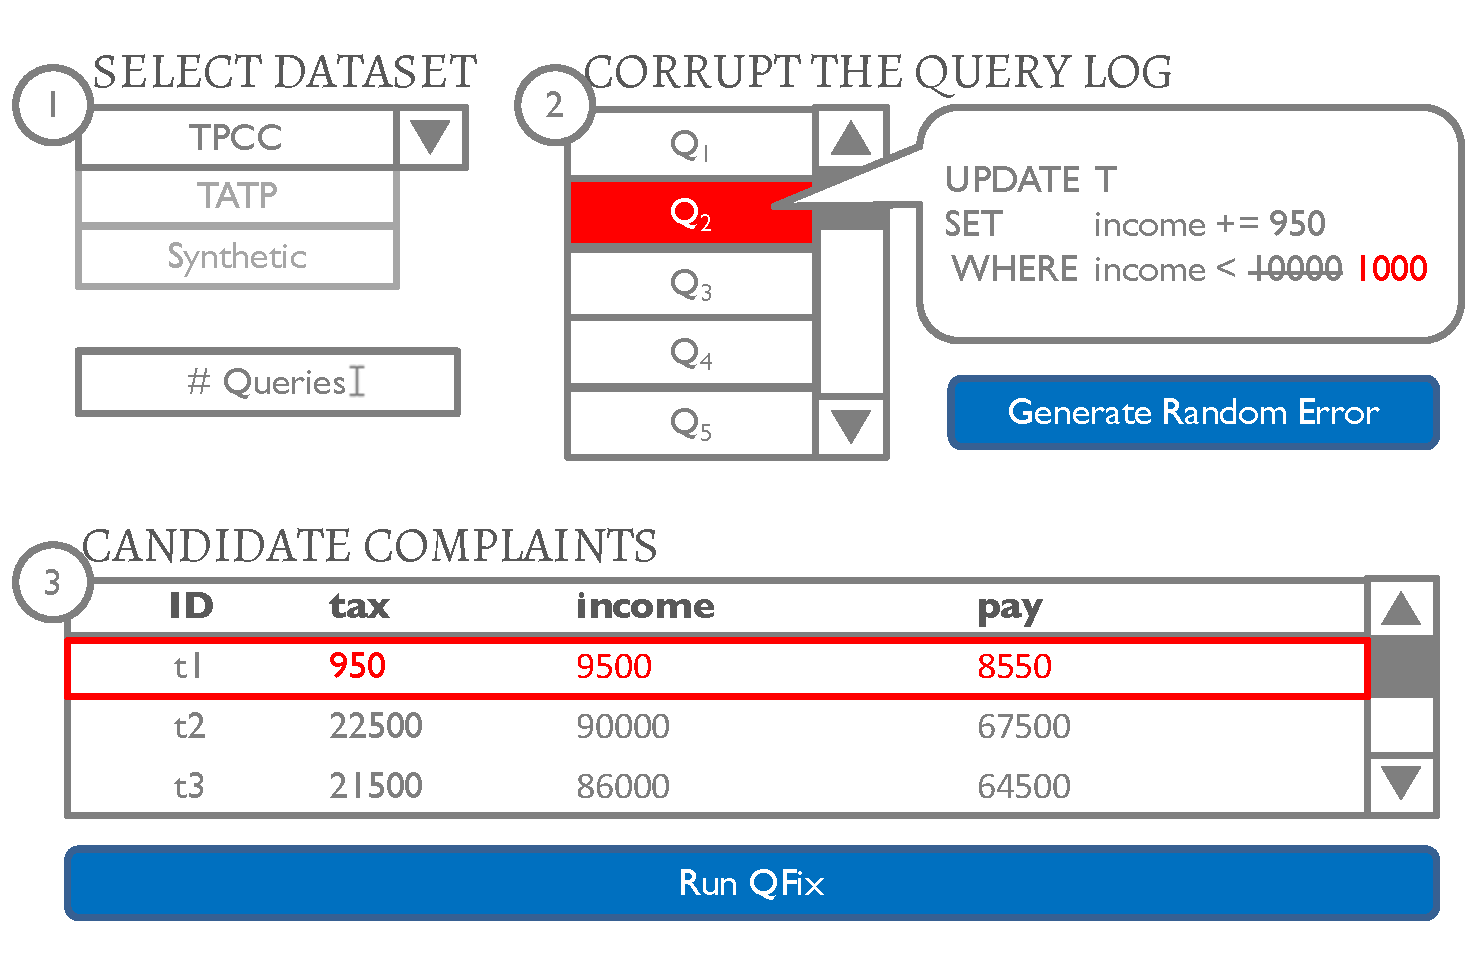
\includegraphics[width = .8\columnwidth]{figures/demo1_exp2}
  \vspace*{-0.2in}
  \caption{Users introduce errors to benchmark workloads.}
  \label{f:demo1} 
  \vspace*{-.3in}
\end{figure}

Figures~\ref{f:demo1} and~\ref{f:demo2} show screenshots of the initial and results pages.
Each step is annotated with a circled number, which we detail below.

\noindent {\bf Step 1 (Select Dataset):} Participants may first choose from a dropdown menu containing
a number of transaction workload generators from the benchmarks in OLTPBench~\cite{oltpbench}.
Since most transactional benchmarks focus on point update queries, we additionally include a 
synthetic workload generator that includes range updates, as well as insert and delete queries.
The text box on the right side allows users to additionally specify the number of queries to generate
in the workload.  

\noindent {\bf Step 2 (Corrupt the Query Log):} 
Once the workload generator is specified, the Query Log component of the interface
renders a scrollable list containing all of the queries.  Users can either let the system to 
inject errors randomly by clicking the ``Random Error'' button or manually add errors. 
To introduce errors, the interface allows users to select any editable query in the log and shows the 
selected query in an editable popup so that users can edit the queries.  
For example, in the figure, the user has edited query $Q_2$ and reduced the threshold from 
$income < 10,000$ to $income < 100$.
%For example, in the figure, the user has edited query $Q_2$ by changing the \texttt{SET}
%clause from $income = 1.1 * income$ to $income = 1.5 * income$. 

\noindent {\bf Step 3 (Form a Complaint Set):} 
The modified query cause the state of the database at the end of the workload
to differ from the result of the original workload.  The candidate complaints table lists the tuples
that are different and highlights the attribute values in those tuples as red text.  For instance,
$t_1.tax$, $t_1.income$ and $t_1.pay$ are all errors introduced by the modified query. 
Users can select individual attribute values or entire tuples to add to the complaint set that is used as input to the \sys algorithms.  
When she is satisfied, the user clicks \texttt{Run QFix} to execute the baseline \sys, the optimized \sys, and alternative algorithms.


\begin{figure}[t]
\centering
  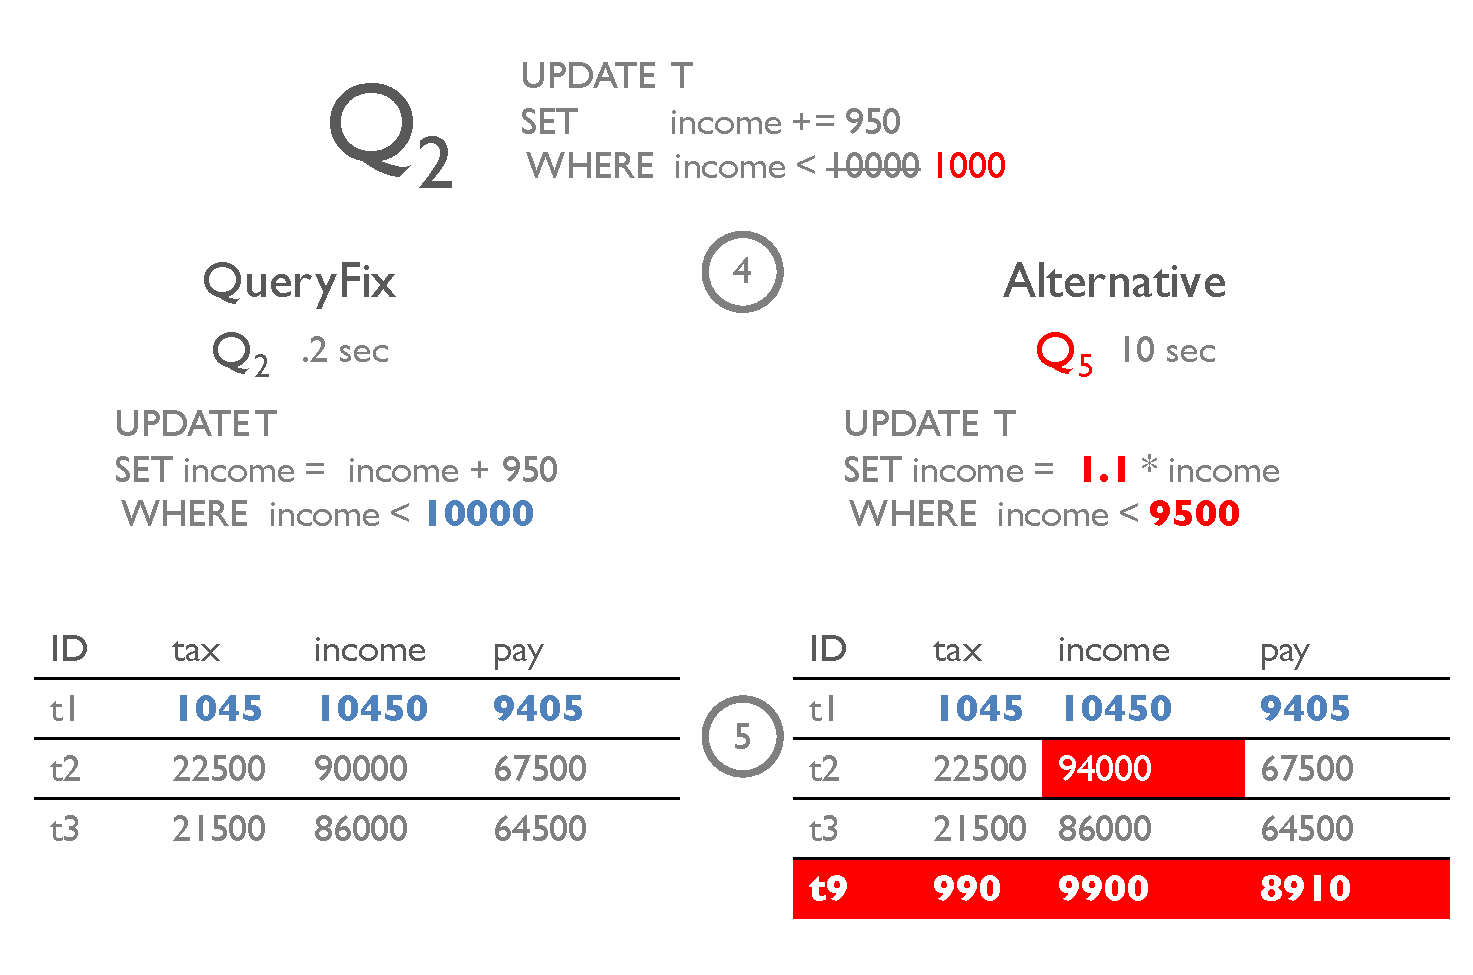
\includegraphics[width = .8\columnwidth]{figures/demo2_exp2}
  \vspace*{-0.2in}
  \caption{Comparisons between proposed fixes.}
  \label{f:demo2} 
  \vspace*{-.2in}
\end{figure}


\noindent {\bf Step 4 (View Log Repairs):}  The result page lists the original query ID and text at the top.  The ID 
is important because some proposed fixes may identify an incorrect query.  Below the original query,
the interface shows each of the proposed fixes as columns.  For example, Figure~\ref{f:demo2} shows 
that both the \sys and alternative fixes identified the correct query $Q_2$, however \sys only took $0.2$ seconds
to run, and correctly fixed $Q_2$, whereas the alternative took $10$ sec, 
incorrectly selected $Q_5$, and proposed an incorrect fix.

\noindent {\bf Step 5 (Validate Repairs):} The bottom tables show the effects of the fixes on the complaints from
step 3.  Correctly fixed attribute values are highlighted in blue, unfixed errors are shown as red text, while incorrectly
fixed values are highlighted with a red background.  Finally, it is possible for proposed fixes to 
{\it introduce} new errors, which are shown as entire rows that are highlighted with a red background.







